\chapter{Riemann Sums}

\section{The Meaning of the Area Under a Function}
%recall hammer toss example, make velocity graph, show area for simple shape, discuss units and meaning

Let's look at the example of a hammer tossed in the air from a previous chapter. As you may recall, if a hammer is tossed up from the ground at 5 m/s, its velocity can be described as $v(t) = 5-9.8t$ (on Earth, where the acceleration due to gravity is approximately $-9.8$ $\frac{m}{s^2}$). The velocity function of our hammer from when it is tossed ($t=0$) to when it hits the ground $t\approx1.02$) is shown in figure \ref{fig:hammer}.

\begin{figure}[htbp]
	\centering
	\begin{tikzpicture}
		\begin{axis}[axis lines = center, xmin=0, xmax=1.02, xlabel=$t$(sec), ymin=-5, ymax=5, ylabel=$v$(m/s)]
		\addplot[blue, smooth, samples=50]{5-9.8*x};
		\end{axis}
	\end{tikzpicture}
	\caption{Velocity of a hammer thrown upwards at 5 m/s}
	\label{fig:hammer}
\end{figure}

Now, suppose we only have this velocity function and we want to know how high above its initial position the hammer is tossed. Examine the graph: at approximately what time does the hammer reach its peak height? (Hint: what should the hammer's velocity be when it reaches its peak?). At the highest point of its flight, the hammer's velocity will be $0$ $\frac{m}{s}$, which occurs at approximately $t=0.5s$ (it's actually $t=0.5102s$ but we don't need to be that precise for this example). 

Now that we know \textit{when} the hammer reaches its peak, how can we determine \textit{how high} that peak is? Recall that velocity is the slope of the position-time graph. Since slope is change in position divided by change in time (in this case, as time is on the $x$-axis and position on the $y$-axis), then the slope must have units of [position]/[time] which could be $\frac{m}{s}$, $\frac{miles}{hr}$, etc. These are units of velocity! 

In figure \ref{fig:hammer}, you can see that the units on the $x$-axis are seconds and on the $y$-axis the units are $\frac{m}{s}$. If we are looking for a \textit{displacement} (that is, how far from its initial position the hammer has traveled), we are looking for a solution with units of meters. To yield an answer with those units, we wouldn't use the slope of the graph: this would yield an answer with units $\frac{m}{s^s}$, the units for acceleration. Instead, we need to \textit{multiply}! The area between the velocity function and the $x$-axis (see figure \ref{fig:hammerarea}) can be found this way:

$$Area=\frac{1}{2}bh$$where b is the base of the triangle and h is the height. 
$$Area=\frac{1}{2}(0.5s)(5\frac{m}{s})$$
$$Area=1.25m$$


%fixme fill not showing in built pdf
\begin{figure}[htbp]
	\centering
	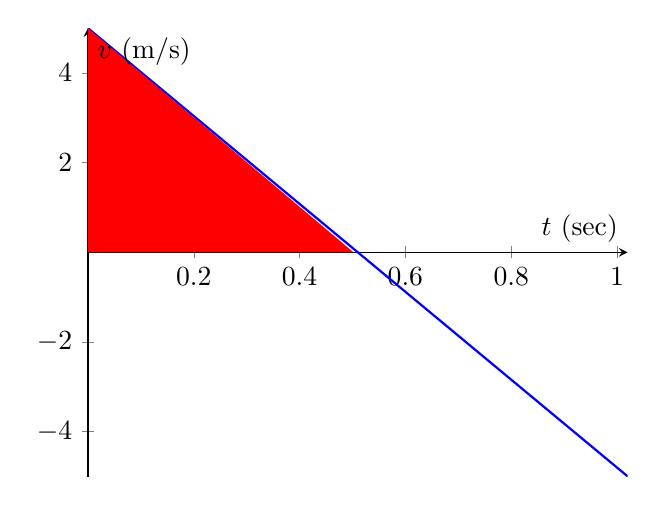
\begin{tikzpicture}
		\begin{axis}[axis lines = center, xmin=0, xmax=1.02, xlabel=$t$ (sec), ymin=-5, ymax=5, ylabel=$v$ (m/s)]
		\addplot[blue, smooth, thick, samples=50]{5-9.8*x};
		\coordinate (c0) at (0,0);
		\coordinate (c1) at (0.502, 0);
		\coordinate (c2) at (0, 5);
		\fill[red] (c0) -- (c1) -- (c2) -- cycle;
		\end{axis}
	\end{tikzpicture}
	\caption{The area under $v(t)$ from $x=0$ to $x=0.5$ is equal to the displacement of the hammer}
	\label{fig:hammerarea}
\end{figure}

Notice that when multiplying the change in time ($0.5$ $s$) by the change in velocity ($1.25$ $\frac{m}{s}$), the seconds units cancel, yielding a result with units of meters. Therefore, the hammer reaches a peak height of $\approx1.25$ $m$, which you can confirm by examining the graph originally presented for the hammer toss in the chapter %blank FIXME reference First and Second derivatives and the shape of functions chapter



\section{Estimating the area under functions}

In the hammer example above, it was easy to determine the area under the function, since the area took the shape of a triangle. But what about finding the area under a more complex function, such as $f(x) = sin{x}+x$ (shown in figure \ref{fig:riemannsine})?

\begin{figure}[htbp]
	\centering
	\begin{tikzpicture}
		\begin{axis}
            [axis lines = center, 
            xmin=0, xmax=3.141592, xlabel=$x$, xtick={0, 0.785398, 1.570796, 2.356194, 3.141593}, xticklabels={$0$, $\frac{\pi}{4}$, $\frac{\pi}{2}$, $\frac{3\pi}{4}$, $\pi$},
            ylabel=$y$, ymin =0, ymax=3.25, ytick={1, 2, 3}, yticklabels={$1$, $2$, $3$}]
			\addplot[blue, samples=50, domain=0:3.141592]{sin(deg(x))+x};
		\end{axis}
	\end{tikzpicture}
	\caption{$f(x) = \sin{x}+x$}
	\label{fig:riemannsine}
\end{figure}

How can we determine the area under $f(x) = \sin{x}+x$ from $x=0$ to $x=\pi$? We can \textit{estimate} the area of that region by dividing the region into rectangles, finding the areas of the rectangles, and adding the areas. As an example, we will divide the region under $f(x) = \sin{x}+x$ into 4 intervals, shown in figure \ref{fig:sinesections}.

\begin{figure}[htbp]
	\centering
	\begin{tikzpicture}
		\begin{axis}[axis lines = center, 
            xmin=0, xmax=3.15, xlabel=$x$, xtick={0, 0.785398, 1.570796, 2.356194, 3.141593}, xticklabels={$0$, $\frac{\pi}{4}$, $\frac{\pi}{2}$, $\frac{3\pi}{4}$, $\pi$},
            ylabel=$y$, ymin =0, ymax=3.25, ytick={1, 2, 3}, yticklabels={$1$, $2$, $3$}]
			\addplot[blue, thick, samples=50, domain=0:6.283185]{sin(deg(x))+x};
                \addplot[black, samples=50]coordinates{(0.785, 0) (0.785, 1.4925)};
                \addplot[black, samples=50]coordinates{(1.570796, 0) (1.570796, 2.5708)};
                \addplot[black, samples=50]coordinates{(2.356194, 0) (2.356194, 3.0633)};
                \addplot[black, samples=50]coordinates{(3.141592, 0) (3.141592, 3.141592)};
		\end{axis}
	\end{tikzpicture}
	\caption{$f(x) = \sin{x}+x$ divided into 4 regions}
	\label{fig:sinesections}
\end{figure}

As you can see in \ref{fig:sinesections}, each rectangle will have a width of $\frac{\pi}{4}$. But what about the height? One way is to use the value of the function at the rightmost value of each rectangle, as shown in figure \ref{fig:sineright}. 

\begin{figure}[htbp]
	\centering
	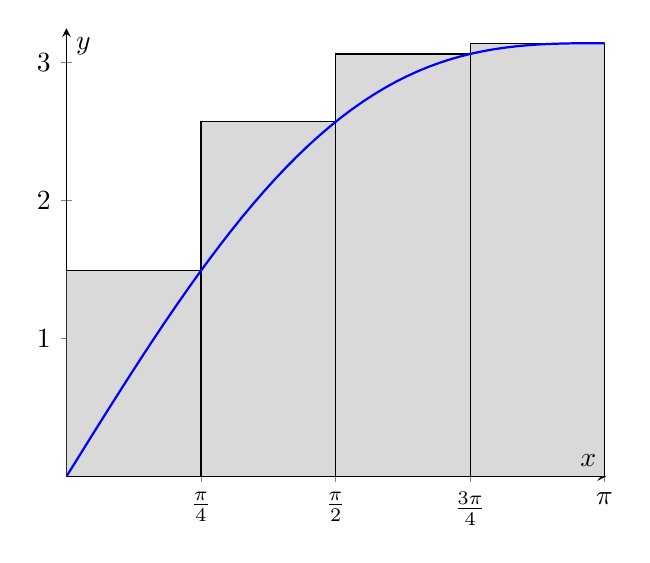
\begin{tikzpicture}
		\begin{axis}[axis lines = center, 
            xmin=0, xmax=3.15, xlabel=$x$, xtick={0, 0.785398, 1.570796, 2.356194, 3.141593}, xticklabels={$0$, $\frac{\pi}{4}$, $\frac{\pi}{2}$, $\frac{3\pi}{4}$, $\pi$},
            ylabel=$y$, ymin =0, ymax=3.25, ytick={1, 2, 3}, yticklabels={$1$, $2$, $3$}]
                \filldraw[fill=gray!30] (0,0) rectangle (0.785, 1.4925);
                \filldraw[fill=gray!30] (0.785398, 0) rectangle (1.570796, 2.5708);
                \filldraw[fill=gray!30] (1.570796, 0) rectangle (2.356194, 3.0633);
                \filldraw[fill=gray!30] (2.356194, 0) rectangle (3.141592, 3.141592);
			\addplot[blue, thick, samples=50, domain=0:3.141592]{sin(deg(x))+x};
		\end{axis}
	\end{tikzpicture}
	\caption{Four rectangle sections with heights determined by rightmost value of $f(x)$ on each interval}
	\label{fig:sineright}
\end{figure}

We can easily calculate the areas of each of these rectangles:
$$\frac{\pi}{4} \times f(\frac{\pi}{4}) + \frac{\pi}{4} \times f(\frac{\pi}{2}) + \frac{\pi}{4} \times  f(\frac{3\pi}{4}) + \frac{\pi}{4} \times f(\pi)$$
$$\approx \frac{\pi}{4} \times (1.4925 + 2.5708 + 3.0633 + 3.1416) = 8.0646$$

Based on figure \ref{fig:sineright}, will the calculated area be an overestimate or an underestimate? Each of the rectangles overshoots the function, so this will be an overestimate. What about using the leftmost value of $f(x)$ of each interval to determine the height of the rectangles? This is shown in figure \ref{fig:sineleft}.

\begin{figure}[htbp]
	\centering
	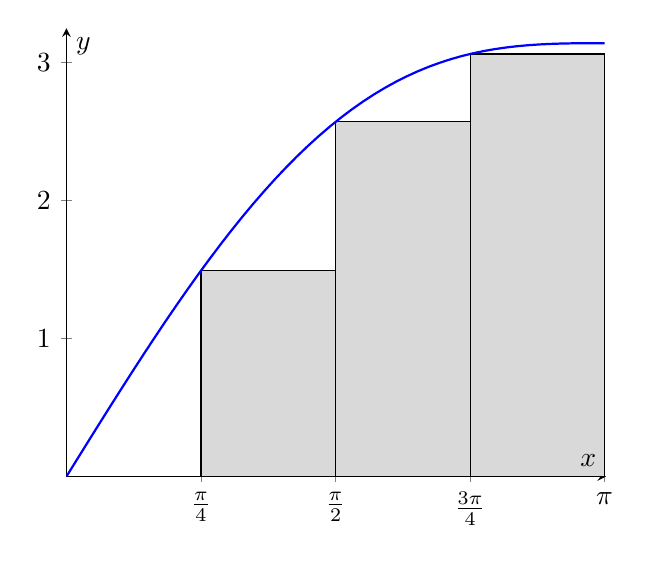
\begin{tikzpicture}
		\begin{axis}[axis lines = center, 
            xmin=0, xmax=3.15, xlabel=$x$, xtick={0, 0.785398, 1.570796, 2.356194, 3.141593}, xticklabels={$0$, $\frac{\pi}{4}$, $\frac{\pi}{2}$, $\frac{3\pi}{4}$, $\pi$},
            ylabel=$y$, ymin =0, ymax=3.25, ytick={1, 2, 3}, yticklabels={$1$, $2$, $3$}]
                \filldraw[fill=gray!30] (0,0) rectangle (0.785, 0);
                \filldraw[fill=gray!30] (0.785398, 0) rectangle (1.570796, 1.4925);
                \filldraw[fill=gray!30] (1.570796, 0) rectangle (2.356194, 2.5708);
                \filldraw[fill=gray!30] (2.356194, 0) rectangle (3.141592, 3.0633);
			\addplot[blue, thick, samples=50, domain=0:3.141592]{sin(deg(x))+x};
		\end{axis}
	\end{tikzpicture}
	\caption{Four rectangle sections with heights determined by leftmost value of $f(x)$ on each interval}
	\label{fig:sineleft}
\end{figure}

Notice that because $f(0)=0$, the height of the first rectangle is zero, so we don't see it on the graph. To find the area of these rectangles:
$$\frac{\pi}{4} \times f(0) + \frac{\pi}{4} \times f(\frac{\pi}{4}) + \frac{\pi}{4} \times f(\frac{\pi}{2}) + \frac{\pi}{4} \times f(\frac{3\pi}{4})$$
$$\approx \frac{\pi}{4} \times (0 + 1.4925 + 2.5708 + 3.0633)=5.5972$$

This is an underestimate. Therefore, the true value of the area under $f(x) = \sin{x} +x$ is between $5.5972$ and $8.0646$. 

\begin{Exercise}[label=rsum1]
	Estimate the area under the graph of $f(x) = \frac{1}{x}$ from $x=1$ to $x=2$ using four rectangles and right endpoints. Sketch the graph and the rectangles. Is your estimate an overestimate or an underestimate? Repeat using left endpoints. 
	\vspace{100mm}
\end{Exercise}

\begin{Answer}[ref=rsum1]

\end{Answer}

\section{The Riemann Sum}
%formal definition, LRM riemann sums with collapsed equations as appropriate
\section{Riemann Sum Examples}

When taking a left Riemann sum, the height of the rectangle is determined by the value of the function at the lower (left-most) $x$-value. See figure \ref{fig:leftriemann}. Based on the graph, do you think a left Riemann sum overestimates or underestimates the area under the curve?

%fixme rectangles show in overleaf but not build%

\begin{figure}
    \centering
    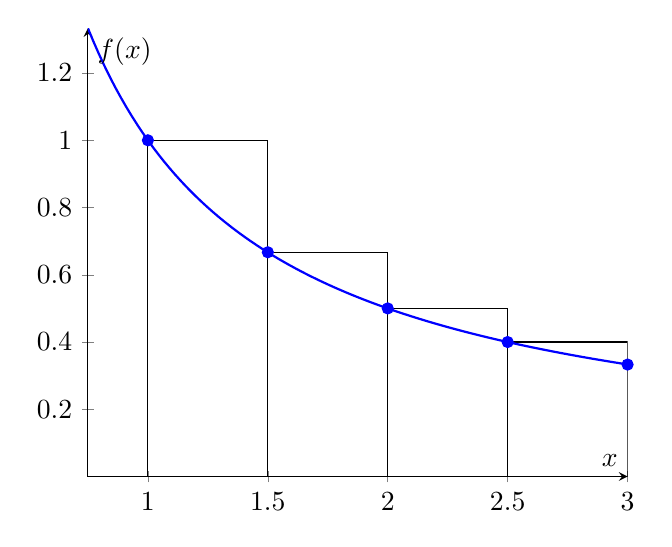
\begin{tikzpicture}
        \begin{axis}[axis lines = center, xmin=0.75, xmax=3, ymin=0, xlabel=$x$, ylabel=$f(x)$]
            \draw (1,0) rectangle (1.5,1);
            \draw (1.5,0) rectangle (2, 0.667);
            \draw (2,0) rectangle (2.5, 0.5);
            \draw (2.5,0) rectangle (3, 0.4);
            \addplot[blue, thick, samples=100, domain=0.75:3]{1/x};
            \addplot[mark=*, blue, only marks]coordinates{(1,1) (1.5,0.667) (2, 0.5) (2.5,.4) (3,0.333)};
        \end{axis}
    \end{tikzpicture}
    \caption{Left Riemann sum of $f(x)=\frac{1}{x}$}
    \label{fig:leftriemann}
\end{figure}

A right Riemann sum uses the right-most value of $f(x)$ to determine the height of the rectangle. As you can see in figure \ref{fig:rightriemann}, right Riemann sums underestimate the area under concave up curves. 

\begin{figure}
    \centering
    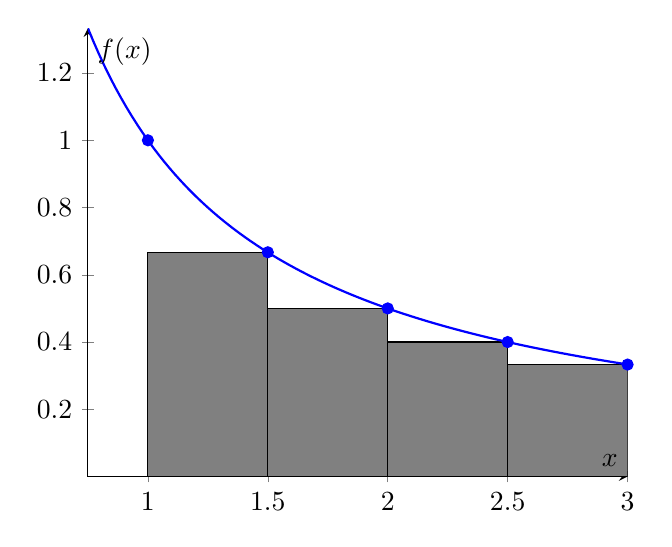
\begin{tikzpicture}
        \begin{axis}[axis lines = center, xmin=0.75, xmax=3, ymin=0, xlabel=$x$, ylabel=$f(x)$]
            \filldraw[fill=gray] (1,0) rectangle (1.5,0.667);
            \filldraw[fill=gray] (1.5,0) rectangle (2, 0.5);
            \filldraw[fill=gray] (2,0) rectangle (2.5, 0.4);
            \filldraw[fill=gray] (2.5,0) rectangle (3, 0.333);
            \addplot[blue, thick, samples=100, domain=0.75:3]{1/x};
            \addplot[mark=*, blue, only marks]coordinates{(1,1) (1.5,0.667) (2, 0.5) (2.5,.4) (3,0.333)};
        \end{axis}
    \end{tikzpicture}
    \caption{Right Riemann sum of $f(x)=\frac{1}{x}$}
    \label{fig:rightriemann}
\end{figure}

A midpoint Riemann sum uses the value of $f(x)$ at the midpoint of the division to determine the height of the rectangle, as shown in figure \ref{fig:midriemann}. 

\begin{figure}
    \centering
    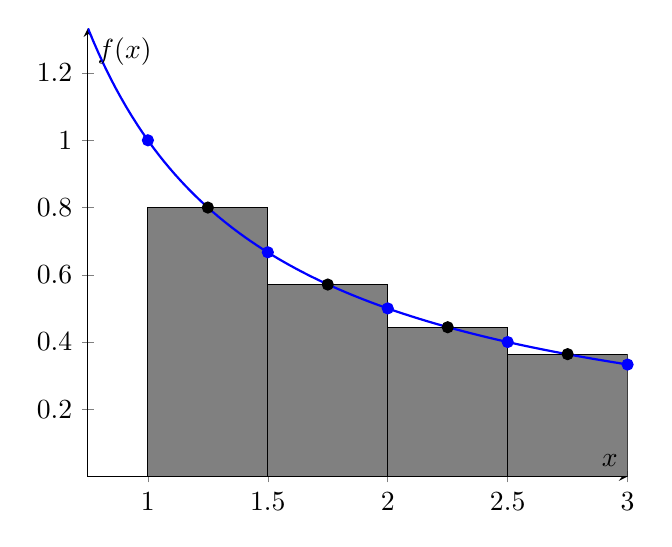
\begin{tikzpicture}
        \begin{axis}[axis lines = center, xmin=0.75, xmax=3, ymin=0, xlabel=$x$, ylabel=$f(x)$]
            \filldraw[fill=gray] (1,0) rectangle (1.5,0.8);
            \filldraw[fill=gray] (1.5,0) rectangle (2, 0.571);
            \filldraw[fill=gray] (2,0) rectangle (2.5, 0.444);
            \filldraw[fill=gray] (2.5,0) rectangle (3, 0.364);
            \addplot[blue, thick, samples=100, domain=0.75:3]{1/x};
            \addplot[mark=*, blue, only marks]coordinates{(1,1) (1.5,0.667) (2, 0.5) (2.5,.4) (3,0.333)};
            \addplot[mark=*, black, only marks]coordinates{(1.25,0.8) (1.75,0.571) (2.25, 0.444) (2.75,.364)};
        \end{axis}
    \end{tikzpicture}
    \caption{Midpoint Riemann sum of $f(x)=\frac{1}{x}$}
    \label{fig:midriemann}
\end{figure}

\section{Code for a Riemann Sum}
%python magic

\section{Riemann Sum Practice}

\begin{Exercise}[label=rsum2]
	\begin{center}
		\begin{tabular}{c|c|c|c|c}
			t (hours) & 4 & 7 & 12 & 15\\
			R(t) (L/hr) & 6.5 & 6.2 & 5.9 & 5.6\\
		\end{tabular}
	\end{center}
	A tank contains 50 liters of water after 4 hours of filling. Water is being added to the tank at rate $R(t)$. The value of $R(t)$ at select times is shown in the table. Using a right Riemann sum, estimate the amount of water in the tank after 15 hours of filling. 
\end{Exercise}

\begin{Answer}[ref=rsum2]
	The volume of water will be the amount of water at 4 hours (50 liters) plus the area under the graph of $R(t)$ from $t=4$ to $t=15$. We will estimate this area with a right Riemann sum. The approximate volume added from $t=4$ to $t=7$ is $(7-4)*(6.2) = 18.6$ liters. The approximate volume added from $t=7$ to $t=12$ is $(12-7)*(5.9)=29.5$ liters. The approximate volume added from $t=12$ to $t=15$ is $(15-12)*(5.6) = 16.8$ liters. Therefore, the approximate total volume of water in the tank at $t=15$ is $50 + 18.6 + 29.5 + 16.8 = 114.9$ liters. 
\end{Answer}